\chapter{\label{cha:glossary}Glossary}

In this appendix we give an overview of frequently used terms and
abbreviations.

\begin{description}
\item[RE:] Reverse Engineer or Reverse Engineering
\item[NMT:] Neural Machine Translation
\item[MASK:] Mask Preditction
\item[DOBF:] Deobfuscation
\item[SPAN:] Span detection
\item[IR:] Intermediate Representation
\item[NLP:] Natural Language Processing
\item[ML:] Machine Learning
\item[CNN: ] Convolutional Neural Network
\item[RNN: ] Recurrent Neural Network
\item[LSTM: ] Long Short-Term Memory
\item[NL: ] Natural Language
\item[PL: ] Programming Language
\item[seq2seq:] Sequence-to-sequence
\item[LLM: ] Large Language Model
\item[BLEU:] BiLingual Evaluation Understudy
\item[EM: ] Exact Match
\item[MLM:] Masked Language Modeling
\item[COTS: ] Commercial Off-The-Shelf
\item[SOTA: ] State-Of-The-Art
\item[TL: ] Transfer Learning
\end{description}

\newpage
\chapter{\label{app:ExtremeSum} Extreme Summarization}
In this appendix we report on the application of the extreme summarization task on our dataset. 

\section{Methodology and Experimental Setup}
We apply the parameters and setup as provided by \citeauthor{PolyglotCodeBERT} for the extreme summarization task \footnote{Model and parameters: \url{https://zenodo.org/record/5670434}}. Note that the authors use their setup for the summarization task and only change the maximum target length of the output to 10 tokens. We fine-tune a CodeBERT \cite{CodeBERT} model for 5 epochs, we chose this limit for brevity as we found that all models converged during the third or fourth epoch \ref{fig:ExtremeLoss}. After every epoch we evaluate the model using the validation set, and finally the model is tested using the test set.

\label{fig:ExtremeLoss}
\begin{figure}[h]
  \centering
  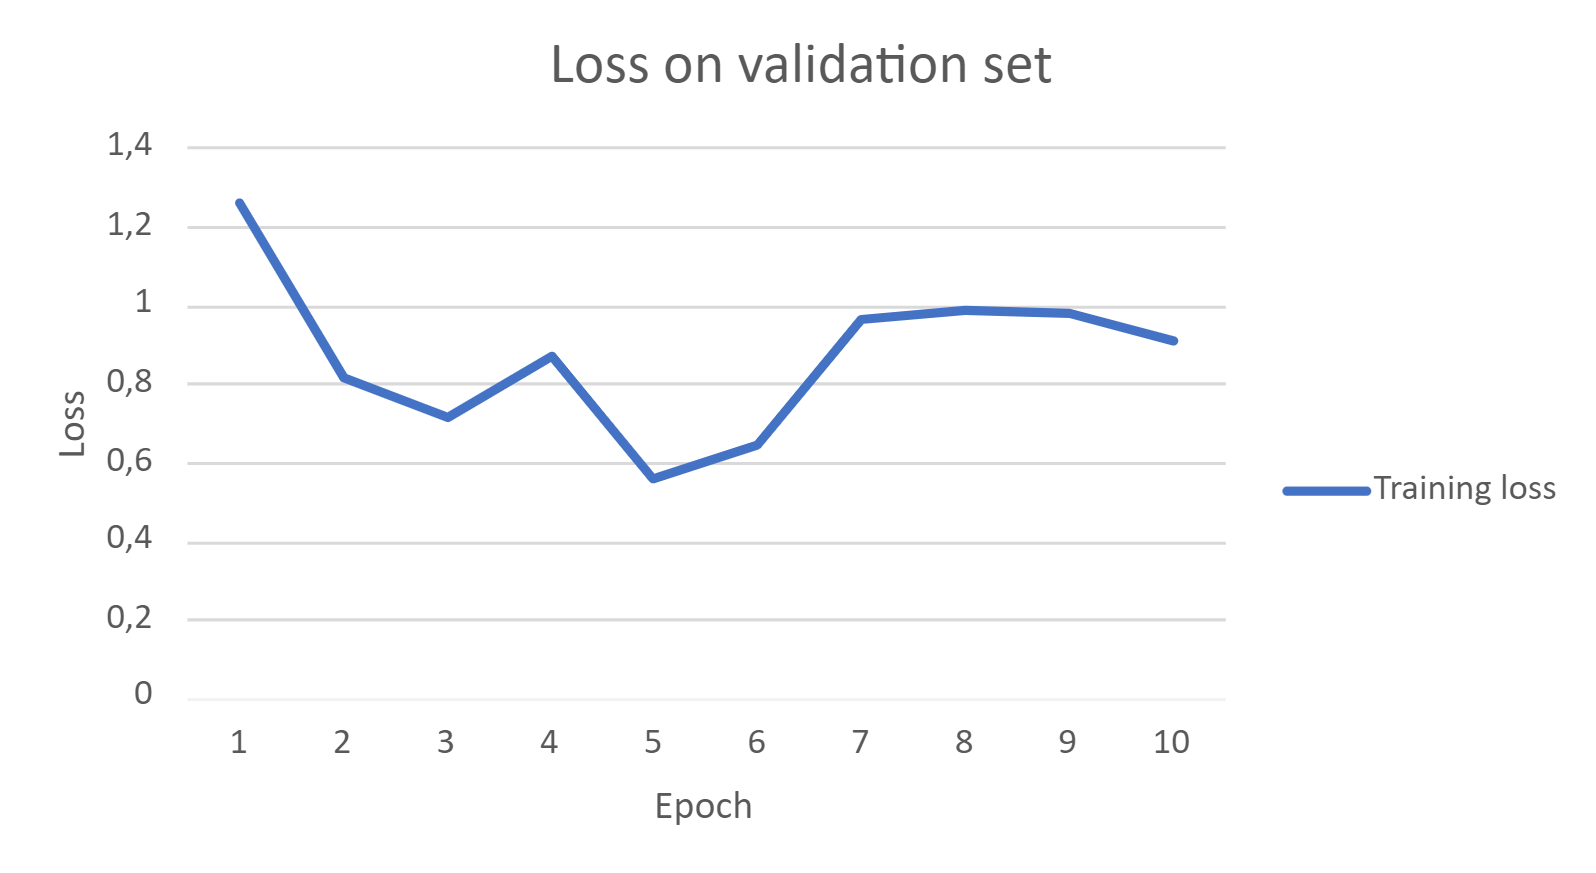
\includegraphics[width=\linewidth]{img/ExtremeLoss.png}
  \caption{Loss during CodeBERT training on stripped data}
\end{figure}

To prepare the dataset, we use the same pipeline as shown in \ref{fig:dataCollection}. Instead of extracting the comment data, the name of the functions is extracted from their aligned source code. These function names will function as reference. Since missing or unalignable documentation is no longer an issue, we are able to collect significantly more decompiled function-function name pairs. Our dataset consists of 2.1m decompiled and 630k stripped samples. Recall that unstripped decompiled functions still retain the function name after decompilation, so we selectively strip away the function name from the function definition and any recursive calls in the function bodies. 

The dataset is split into a train, test and validation set. Similarly to the regular summarization task we split them in a cross-project manner, with the sets constituting 80\%, 10\% and 10\% of the complete dataset respectively. We followed the recommendations by  \citeauthor{recommend_summarization} on the dataset construction. 

Since the output of the model is so short and generally contains up to 3 tokens \cite{ExtremeSummarization}, BLEU would be unfit as a metric. Similarly to \citeauthor{ExtremeSummarization} and \citeauthor{PolyglotCodeBERT}, we chose to use the F1-score.
\[F1 = \frac{2*Precision*Recall}{Precision+Recall}\] 
Every function name is broken up into subtokens, the name "popStack" would therefore be tokenized into "pop" and "stack". The precision and recall are then calculated by comparing the tokens in the anchor and the model prediction. Note that this does not take the order of the tokens into account.

\citeauthor{PolyglotCodeBERT} report F1 scores ranging from 0.24 to 0.54 and F1 scores ranging from 0.41 and 0.54 with regular CodeBERT and PolyglotCodeBERT respectively. Note that these models were trained and evaluated on the CodeXGLUE \cite{CodeXGlue} dataset which is deduplicated, while our own dataset is not. %Find limit for unusable samples

\section{Results}
We found that the results resembled the results from the regular code summarization task. The CodeBERT model achieved an F1 score of 20.6 and 5.45 on the stripped and unstripped code respectively. Manual assessment of the produced samples shows that the model for unstripped code could produce some useable samples, but the stripped model was unable to produce almost anything of value.

\begin{table}[h]
\begin{tabular}{l|ll}
\multicolumn{1}{c|}{Reference} & \multicolumn{1}{c}{Decom} & \multicolumn{1}{c}{Stripped} \\ \hline
main                           & main                      & main                         \\
sha 256 transform              & md 5  process  block      & sha 1  process  block        \\
get ins len                    & op nd  num  reg s         & op nd  get  size             \\
r id storage foreach           & queue  fore ach           & hash  find                   \\
map init                       & pro g  init               & c se g  open                
\end{tabular}
\caption{Sample of CodeBERT extreme summarization model output}
\end{table}


% \newpage
% \chapter{\label{app:Dataset} Dataset}